\documentclass[portrait]{seminar}
\usepackage{epic,eepic,colordvi,psfig}
\background{White}
\textBlack
\portraitonly
\slideframe{none}
\paperheight 20.2cm
\paperwidth 27cm
\renewcommand\slideleftmargin{-7.1cm}
\begin{document}

\title{{Military Impact of  F30602-97-1-0205}}
\author{ \\ 
\\
\\
\\
\Green{Yvo Desmedt\\
Department of EE \& CS\\
University of Wisconsin---Milwaukee\\
{\tt desmedt@cs.uwm.edu}
}}

\maketitle

\newpage

\section*{\Green{Overview}}

\Red{
\begin{itemize}
\item State of the art
\item Security aspects overlooked
\item Importance of the aspects to the military
\item Obtained results
\item Potential impact
\item Future plans
\end{itemize}
}
\newpage

\section*{\Red{State of the art}}

Redundancy is used to: 

\begin{itemize}
\item increase fault-tolerance
\item protect against $k$ adversaries
\end{itemize}
in such applications as:

\begin{itemize}
\item communication (error-correcting codes)
\item networks
\begin{itemize}
\item against destructing nodes and edges: needs $k+1$-connected

\vskip 10pt
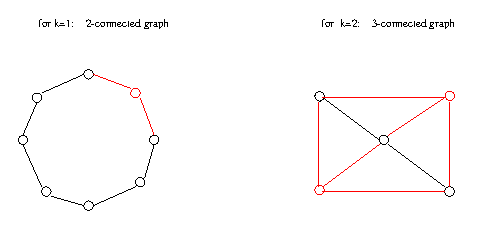
\psfig{file=slidepic1.eps}


\item against Byzantine (lying) nodes: needs $2k+1$-connected

\vskip 10pt
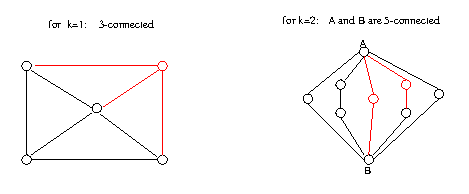
\psfig{file=slidepic2.eps}

\end{itemize}
\item distributed computer environment
\begin{itemize}
\item computers being destructed
\item computers being taken over by the enemy
\end{itemize}
\end{itemize}


\newpage
\section*{\Red{Security aspects overlooked}}

\begin{itemize}
\item \Blue{Current network results}

Only the following has been discussed:
\begin{itemize}
\item The network is known 

{\small E.g., Dovev, Dwork, Waarts, and  Yung $[1993]$,
Franklin and Wright $[1998]$}
\item The network is known and there are no malicious
errors 

{\small E.g., flooding, shortest paths}
\item There is a trusted \underline{\Green{central}}
certification authority and a supernetowrk is known

{\small E.g., Radia Perlman}
\end{itemize}

Missing:
\begin{itemize}
\item Unknown network $+$ malicious faults.

\vskip 10pt
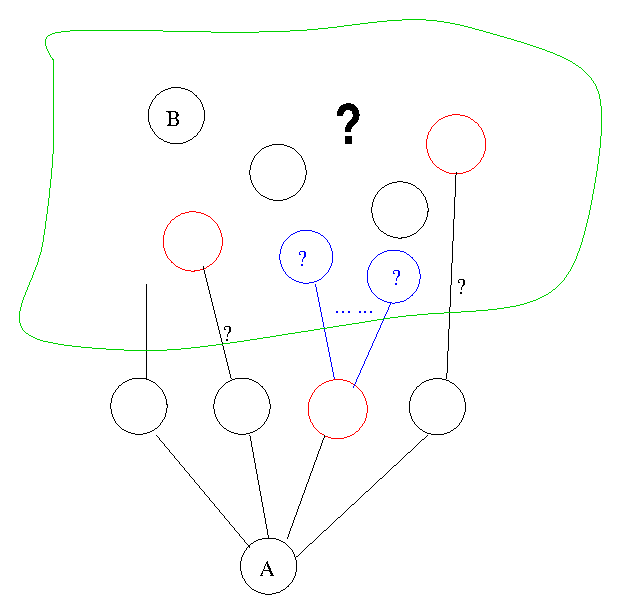
\psfig{file=slidepic3.eps}
\end{itemize}
Note: A node can make $\infty$ many bogus nodes and edges.


\item \Blue{Computer Security}

Programmers: flow chart (different types of inputs).

\Red{A simple example}:
The airplane's next position is decided by
the airplane's current position, the speed, and the
acceleration. More specifically, 
$s=s_0+v\times t+\frac{1}{2}a\times t^2 \ (a=0)$.

$$\begin{array}{ll}
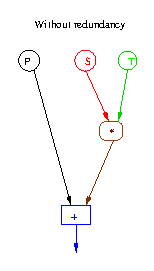
\psfig{file=slidepic4.eps} &
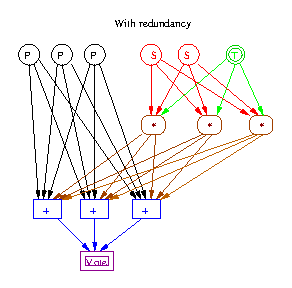
\psfig{file=slidepic5.eps}
\end{array}$$

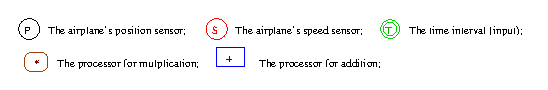
\psfig{file=slidepic6.eps}

\vskip 10pt
Note: \begin{enumerate}
\item for computer networks: efficient algorithms
\item for computer security: {\bf NP}-hardness (our results)
\end{enumerate}
\end{itemize}


\newpage
\section*{\Red{Importance of the aspects to the military}}

\begin{itemize}
\item\Blue{Large networks are unknown}

\end{itemize}


\newpage
\section*{\Red{Obtained results}}

\begin{itemize}
\item\Blue{Network security}

In the context of unknown networks, rooting algorithms 
for the following cases have been obtained:
\begin{itemize}
\item the sender knows the network, but the receiver does not.
\item each node has a public key.
\end{itemize}

\item\Blue{Computer security}
\begin{itemize}
\item modeling redundant multi-input computation: AND/OR graphs.
\item multi-input redundant computation is very different 
from network security.  The following results have demonstrated this:
\begin{itemize}
\item finding disjoint ``paths'' (solution graphs) is {\bf NP}-hard.
\item a smaller number of disjoint paths is sufficient. 
\end{itemize}
\item finding a critical path: a generalization of the
critical paths in PERT graphs.
\item finding critical vertices in an AND/OR graph is 
``harder''.
\end{itemize}


\item\Blue{Other results}
\begin{itemize}
\item Broadcast network

Franklin-Yung (1995) introduced the problem of Byzantine
faults in a broadcast network. Franklin-Wright (1998) shows
that ``broadcasting'' \Green{hurts} adversaries in certain situation.
However, their solution is efficient (exponential) when
$k<n\le  \frac{3}{2}\times k$. We have given a 
efficient solution to this problem. Our results also
shows that in other situations, ``broadcasting'' 
\Green{helps} adversaries.

\item Redundancy to increase efficiency

For the maximal flows in an AND/OR graph, the solution depends 
whether data is processed (which can be copied) or goods (which 
cannot be copied).

\end{itemize}
\end{itemize}

\newpage
\section*{\Red{Potential impact}}

\begin{itemize}
\item One can plan military defenses
with the properties that it is hard for the enemy to find  appropriate
sites to attack such that the damage is maximal.

\item  Evaluating the success 
of a given military strike (or defense)
against an enemy with a number of units is hard.

\item One can design a military strike and a defense
such that the enemy will exhaust some of his units.

\end{itemize}

\newpage
\section*{\Red{Future plans}}

\begin{itemize}
\item\Blue{Plan here}

\end{itemize}

\end{document}


